% Created by tikzDevice version 0.12 on 2019-07-24 15:39:22
% !TEX encoding = UTF-8 Unicode
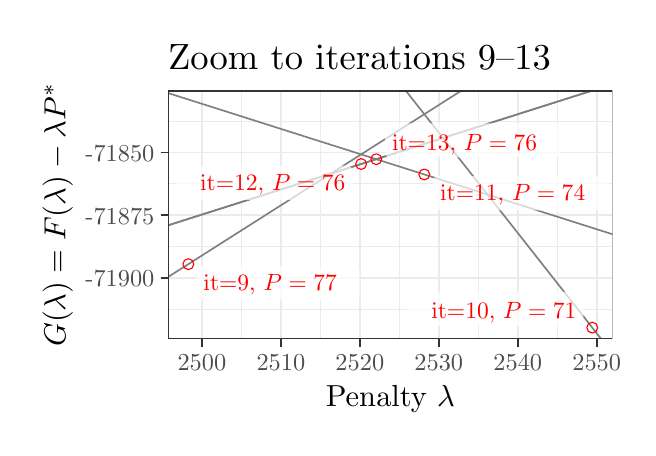
\begin{tikzpicture}[x=1pt,y=1pt]
\definecolor{fillColor}{RGB}{255,255,255}
\path[use as bounding box,fill=fillColor,fill opacity=0.00] (0,0) rectangle (216.81,144.54);
\begin{scope}
\path[clip] (  0.00,  0.00) rectangle (216.81,144.54);
\definecolor{drawColor}{RGB}{255,255,255}
\definecolor{fillColor}{RGB}{255,255,255}

\path[draw=drawColor,line width= 0.6pt,line join=round,line cap=round,fill=fillColor] ( -0.00,  0.00) rectangle (216.81,144.54);
\end{scope}
\begin{scope}
\path[clip] ( 50.75, 32.08) rectangle (211.31,121.66);
\definecolor{fillColor}{RGB}{255,255,255}

\path[fill=fillColor] ( 50.75, 32.08) rectangle (211.31,121.66);
\definecolor{drawColor}{gray}{0.92}

\path[draw=drawColor,line width= 0.3pt,line join=round] ( 50.75, 42.80) --
	(211.31, 42.80);

\path[draw=drawColor,line width= 0.3pt,line join=round] ( 50.75, 65.47) --
	(211.31, 65.47);

\path[draw=drawColor,line width= 0.3pt,line join=round] ( 50.75, 88.13) --
	(211.31, 88.13);

\path[draw=drawColor,line width= 0.3pt,line join=round] ( 50.75,110.79) --
	(211.31,110.79);

\path[draw=drawColor,line width= 0.3pt,line join=round] ( 77.23, 32.08) --
	( 77.23,121.66);

\path[draw=drawColor,line width= 0.3pt,line join=round] (105.76, 32.08) --
	(105.76,121.66);

\path[draw=drawColor,line width= 0.3pt,line join=round] (134.29, 32.08) --
	(134.29,121.66);

\path[draw=drawColor,line width= 0.3pt,line join=round] (162.83, 32.08) --
	(162.83,121.66);

\path[draw=drawColor,line width= 0.3pt,line join=round] (191.36, 32.08) --
	(191.36,121.66);

\path[draw=drawColor,line width= 0.6pt,line join=round] ( 50.75, 54.13) --
	(211.31, 54.13);

\path[draw=drawColor,line width= 0.6pt,line join=round] ( 50.75, 76.80) --
	(211.31, 76.80);

\path[draw=drawColor,line width= 0.6pt,line join=round] ( 50.75, 99.46) --
	(211.31, 99.46);

\path[draw=drawColor,line width= 0.6pt,line join=round] ( 62.96, 32.08) --
	( 62.96,121.66);

\path[draw=drawColor,line width= 0.6pt,line join=round] ( 91.50, 32.08) --
	( 91.50,121.66);

\path[draw=drawColor,line width= 0.6pt,line join=round] (120.03, 32.08) --
	(120.03,121.66);

\path[draw=drawColor,line width= 0.6pt,line join=round] (148.56, 32.08) --
	(148.56,121.66);

\path[draw=drawColor,line width= 0.6pt,line join=round] (177.09, 32.08) --
	(177.09,121.66);

\path[draw=drawColor,line width= 0.6pt,line join=round] (205.62, 32.08) --
	(205.62,121.66);
\definecolor{drawColor}{gray}{0.50}

\path[draw=drawColor,line width= 0.6pt,line join=round] ( 50.75, 54.45) -- (192.54,144.54);

\path[draw=drawColor,line width= 0.6pt,line join=round] (118.72,144.54) -- (211.31, 26.88);

\path[draw=drawColor,line width= 0.6pt,line join=round] ( 50.75,120.91) -- (211.31, 69.90);

\path[draw=drawColor,line width= 0.6pt,line join=round] ( 50.75, 73.12) -- (211.31,124.13);

\path[draw=drawColor,line width= 0.6pt,line join=round] ( 50.75, 73.12) -- (211.31,124.13);
\definecolor{fillColor}{RGB}{255,255,255}

\path[fill=fillColor,fill opacity=0.70] ( 62.81, 46.14) --
	(118.18, 46.14) --
	(118.11, 46.14) --
	(118.40, 46.15) --
	(118.68, 46.21) --
	(118.95, 46.31) --
	(119.20, 46.46) --
	(119.43, 46.64) --
	(119.62, 46.86) --
	(119.78, 47.10) --
	(119.89, 47.37) --
	(119.96, 47.65) --
	(119.98, 47.94) --
	(119.98, 47.94) --
	(119.98, 56.66) --
	(119.98, 56.66) --
	(119.96, 56.95) --
	(119.89, 57.23) --
	(119.78, 57.50) --
	(119.62, 57.75) --
	(119.43, 57.96) --
	(119.20, 58.15) --
	(118.95, 58.29) --
	(118.68, 58.40) --
	(118.40, 58.45) --
	(118.18, 58.47) --
	( 62.81, 58.47) --
	( 63.03, 58.45) --
	( 62.73, 58.47) --
	( 62.45, 58.43) --
	( 62.17, 58.35) --
	( 61.90, 58.23) --
	( 61.66, 58.06) --
	( 61.46, 57.86) --
	( 61.28, 57.63) --
	( 61.15, 57.37) --
	( 61.05, 57.09) --
	( 61.01, 56.81) --
	( 61.00, 56.66) --
	( 61.00, 47.94) --
	( 61.01, 48.09) --
	( 61.01, 47.80) --
	( 61.05, 47.51) --
	( 61.15, 47.23) --
	( 61.28, 46.98) --
	( 61.46, 46.74) --
	( 61.66, 46.54) --
	( 61.90, 46.38) --
	( 62.17, 46.25) --
	( 62.45, 46.17) --
	( 62.73, 46.14) --
	cycle;
\end{scope}
\begin{scope}
\path[clip] ( 50.75, 32.08) rectangle (211.31,121.66);
\definecolor{drawColor}{RGB}{255,0,0}

\node[text=drawColor,anchor=base west,inner sep=0pt, outer sep=0pt, scale=  0.85] at ( 63.53, 49.63) {it=9, $P=77$};
\definecolor{fillColor}{RGB}{255,255,255}

\path[fill=fillColor,fill opacity=0.70] (138.98, 36.77) --
	(199.02, 36.77) --
	(198.95, 36.77) --
	(199.24, 36.78) --
	(199.53, 36.84) --
	(199.80, 36.95) --
	(200.05, 37.09) --
	(200.27, 37.28) --
	(200.47, 37.49) --
	(200.62, 37.74) --
	(200.74, 38.01) --
	(200.81, 38.29) --
	(200.83, 38.58) --
	(200.83, 38.58) --
	(200.83, 47.30) --
	(200.83, 47.30) --
	(200.81, 47.59) --
	(200.74, 47.87) --
	(200.62, 48.14) --
	(200.47, 48.38) --
	(200.27, 48.60) --
	(200.05, 48.78) --
	(199.80, 48.93) --
	(199.53, 49.03) --
	(199.24, 49.09) --
	(199.02, 49.10) --
	(138.98, 49.10) --
	(139.20, 49.09) --
	(138.91, 49.10) --
	(138.62, 49.07) --
	(138.34, 48.99) --
	(138.07, 48.86) --
	(137.84, 48.70) --
	(137.63, 48.49) --
	(137.45, 48.26) --
	(137.32, 48.00) --
	(137.22, 47.73) --
	(137.18, 47.44) --
	(137.17, 47.30) --
	(137.17, 38.58) --
	(137.18, 38.72) --
	(137.18, 38.43) --
	(137.22, 38.15) --
	(137.32, 37.87) --
	(137.45, 37.61) --
	(137.63, 37.38) --
	(137.84, 37.18) --
	(138.07, 37.01) --
	(138.34, 36.89) --
	(138.62, 36.81) --
	(138.91, 36.77) --
	cycle;
\end{scope}
\begin{scope}
\path[clip] ( 50.75, 32.08) rectangle (211.31,121.66);
\definecolor{drawColor}{RGB}{255,0,0}

\node[text=drawColor,anchor=base east,inner sep=0pt, outer sep=0pt, scale=  0.85] at (198.30, 39.30) {it=10, $P=71$};
\definecolor{fillColor}{RGB}{255,255,255}

\path[fill=fillColor,fill opacity=0.70] (148.32, 78.55) --
	(208.36, 78.55) --
	(208.29, 78.55) --
	(208.58, 78.56) --
	(208.87, 78.62) --
	(209.14, 78.72) --
	(209.39, 78.87) --
	(209.62, 79.05) --
	(209.81, 79.27) --
	(209.96, 79.51) --
	(210.08, 79.78) --
	(210.15, 80.06) --
	(210.17, 80.35) --
	(210.17, 80.35) --
	(210.17, 89.07) --
	(210.17, 89.07) --
	(210.15, 89.36) --
	(210.08, 89.64) --
	(209.96, 89.91) --
	(209.81, 90.16) --
	(209.62, 90.38) --
	(209.39, 90.56) --
	(209.14, 90.70) --
	(208.87, 90.81) --
	(208.58, 90.87) --
	(208.36, 90.88) --
	(148.32, 90.88) --
	(148.54, 90.87) --
	(148.25, 90.88) --
	(147.96, 90.84) --
	(147.68, 90.76) --
	(147.42, 90.64) --
	(147.18, 90.47) --
	(146.97, 90.27) --
	(146.79, 90.04) --
	(146.66, 89.78) --
	(146.57, 89.50) --
	(146.52, 89.22) --
	(146.51, 89.07) --
	(146.51, 80.35) --
	(146.52, 80.50) --
	(146.52, 80.21) --
	(146.57, 79.92) --
	(146.66, 79.65) --
	(146.79, 79.39) --
	(146.97, 79.16) --
	(147.18, 78.95) --
	(147.42, 78.79) --
	(147.68, 78.66) --
	(147.96, 78.58) --
	(148.25, 78.55) --
	cycle;
\end{scope}
\begin{scope}
\path[clip] ( 50.75, 32.08) rectangle (211.31,121.66);
\definecolor{drawColor}{RGB}{255,0,0}

\node[text=drawColor,anchor=base west,inner sep=0pt, outer sep=0pt, scale=  0.85] at (149.04, 82.04) {it=11, $P=74$};
\definecolor{fillColor}{RGB}{255,255,255}

\path[fill=fillColor,fill opacity=0.70] ( 55.45, 82.32) --
	(115.49, 82.32) --
	(115.42, 82.32) --
	(115.71, 82.34) --
	(116.00, 82.39) --
	(116.27, 82.50) --
	(116.52, 82.64) --
	(116.75, 82.83) --
	(116.94, 83.04) --
	(117.09, 83.29) --
	(117.21, 83.56) --
	(117.28, 83.84) --
	(117.30, 84.13) --
	(117.30, 84.13) --
	(117.30, 92.85) --
	(117.30, 92.85) --
	(117.28, 93.14) --
	(117.21, 93.42) --
	(117.09, 93.69) --
	(116.94, 93.93) --
	(116.75, 94.15) --
	(116.52, 94.33) --
	(116.27, 94.48) --
	(116.00, 94.58) --
	(115.71, 94.64) --
	(115.49, 94.65) --
	( 55.45, 94.65) --
	( 55.67, 94.64) --
	( 55.38, 94.65) --
	( 55.09, 94.62) --
	( 54.81, 94.54) --
	( 54.55, 94.41) --
	( 54.31, 94.25) --
	( 54.10, 94.05) --
	( 53.92, 93.81) --
	( 53.79, 93.56) --
	( 53.70, 93.28) --
	( 53.65, 92.99) --
	( 53.64, 92.85) --
	( 53.64, 84.13) --
	( 53.65, 84.27) --
	( 53.65, 83.98) --
	( 53.70, 83.70) --
	( 53.79, 83.42) --
	( 53.92, 83.16) --
	( 54.10, 82.93) --
	( 54.31, 82.73) --
	( 54.55, 82.56) --
	( 54.81, 82.44) --
	( 55.09, 82.36) --
	( 55.38, 82.32) --
	cycle;
\end{scope}
\begin{scope}
\path[clip] ( 50.75, 32.08) rectangle (211.31,121.66);
\definecolor{drawColor}{RGB}{255,0,0}

\node[text=drawColor,anchor=base east,inner sep=0pt, outer sep=0pt, scale=  0.85] at (114.77, 85.82) {it=12, $P=76$};
\definecolor{fillColor}{RGB}{255,255,255}

\path[fill=fillColor,fill opacity=0.70] (130.96, 97.63) --
	(191.00, 97.63) --
	(190.93, 97.63) --
	(191.22, 97.64) --
	(191.50, 97.70) --
	(191.77, 97.80) --
	(192.03, 97.95) --
	(192.25, 98.13) --
	(192.44, 98.35) --
	(192.60, 98.60) --
	(192.71, 98.86) --
	(192.78, 99.15) --
	(192.81, 99.44) --
	(192.81, 99.44) --
	(192.81,108.15) --
	(192.81,108.15) --
	(192.78,108.44) --
	(192.71,108.73) --
	(192.60,108.99) --
	(192.44,109.24) --
	(192.25,109.46) --
	(192.03,109.64) --
	(191.77,109.79) --
	(191.50,109.89) --
	(191.22,109.95) --
	(191.00,109.96) --
	(130.96,109.96) --
	(131.17,109.95) --
	(130.88,109.96) --
	(130.59,109.92) --
	(130.31,109.84) --
	(130.05,109.72) --
	(129.81,109.55) --
	(129.60,109.35) --
	(129.43,109.12) --
	(129.29,108.86) --
	(129.20,108.59) --
	(129.15,108.30) --
	(129.15,108.15) --
	(129.15, 99.44) --
	(129.15, 99.58) --
	(129.15, 99.29) --
	(129.20, 99.00) --
	(129.29, 98.73) --
	(129.43, 98.47) --
	(129.60, 98.24) --
	(129.81, 98.04) --
	(130.05, 97.87) --
	(130.31, 97.75) --
	(130.59, 97.67) --
	(130.88, 97.63) --
	cycle;
\end{scope}
\begin{scope}
\path[clip] ( 50.75, 32.08) rectangle (211.31,121.66);
\definecolor{drawColor}{RGB}{255,0,0}

\node[text=drawColor,anchor=base west,inner sep=0pt, outer sep=0pt, scale=  0.85] at (131.67,100.15) {it=13, $P=76$};

\path[draw=drawColor,line width= 0.4pt,line join=round,line cap=round] ( 58.05, 59.08) circle (  1.96);

\path[draw=drawColor,line width= 0.4pt,line join=round,line cap=round] (204.01, 36.15) circle (  1.96);

\path[draw=drawColor,line width= 0.4pt,line join=round,line cap=round] (143.33, 91.50) circle (  1.96);

\path[draw=drawColor,line width= 0.4pt,line join=round,line cap=round] (120.48, 95.27) circle (  1.96);

\path[draw=drawColor,line width= 0.4pt,line join=round,line cap=round] (125.97, 97.01) circle (  1.96);
\definecolor{drawColor}{gray}{0.20}

\path[draw=drawColor,line width= 0.6pt,line join=round,line cap=round] ( 50.75, 32.08) rectangle (211.31,121.66);
\end{scope}
\begin{scope}
\path[clip] (  0.00,  0.00) rectangle (216.81,144.54);
\definecolor{drawColor}{gray}{0.30}

\node[text=drawColor,anchor=base east,inner sep=0pt, outer sep=0pt, scale=  0.88] at ( 45.80, 50.88) {-71900};

\node[text=drawColor,anchor=base east,inner sep=0pt, outer sep=0pt, scale=  0.88] at ( 45.80, 73.54) {-71875};

\node[text=drawColor,anchor=base east,inner sep=0pt, outer sep=0pt, scale=  0.88] at ( 45.80, 96.21) {-71850};
\end{scope}
\begin{scope}
\path[clip] (  0.00,  0.00) rectangle (216.81,144.54);
\definecolor{drawColor}{gray}{0.20}

\path[draw=drawColor,line width= 0.6pt,line join=round] ( 48.00, 54.13) --
	( 50.75, 54.13);

\path[draw=drawColor,line width= 0.6pt,line join=round] ( 48.00, 76.80) --
	( 50.75, 76.80);

\path[draw=drawColor,line width= 0.6pt,line join=round] ( 48.00, 99.46) --
	( 50.75, 99.46);
\end{scope}
\begin{scope}
\path[clip] (  0.00,  0.00) rectangle (216.81,144.54);
\definecolor{drawColor}{gray}{0.20}

\path[draw=drawColor,line width= 0.6pt,line join=round] ( 62.96, 29.33) --
	( 62.96, 32.08);

\path[draw=drawColor,line width= 0.6pt,line join=round] ( 91.50, 29.33) --
	( 91.50, 32.08);

\path[draw=drawColor,line width= 0.6pt,line join=round] (120.03, 29.33) --
	(120.03, 32.08);

\path[draw=drawColor,line width= 0.6pt,line join=round] (148.56, 29.33) --
	(148.56, 32.08);

\path[draw=drawColor,line width= 0.6pt,line join=round] (177.09, 29.33) --
	(177.09, 32.08);

\path[draw=drawColor,line width= 0.6pt,line join=round] (205.62, 29.33) --
	(205.62, 32.08);
\end{scope}
\begin{scope}
\path[clip] (  0.00,  0.00) rectangle (216.81,144.54);
\definecolor{drawColor}{gray}{0.30}

\node[text=drawColor,anchor=base,inner sep=0pt, outer sep=0pt, scale=  0.88] at ( 62.96, 20.63) {2500};

\node[text=drawColor,anchor=base,inner sep=0pt, outer sep=0pt, scale=  0.88] at ( 91.50, 20.63) {2510};

\node[text=drawColor,anchor=base,inner sep=0pt, outer sep=0pt, scale=  0.88] at (120.03, 20.63) {2520};

\node[text=drawColor,anchor=base,inner sep=0pt, outer sep=0pt, scale=  0.88] at (148.56, 20.63) {2530};

\node[text=drawColor,anchor=base,inner sep=0pt, outer sep=0pt, scale=  0.88] at (177.09, 20.63) {2540};

\node[text=drawColor,anchor=base,inner sep=0pt, outer sep=0pt, scale=  0.88] at (205.62, 20.63) {2550};
\end{scope}
\begin{scope}
\path[clip] (  0.00,  0.00) rectangle (216.81,144.54);
\definecolor{drawColor}{RGB}{0,0,0}

\node[text=drawColor,anchor=base,inner sep=0pt, outer sep=0pt, scale=  1.10] at (131.03,  7.62) {Penalty $\lambda$};
\end{scope}
\begin{scope}
\path[clip] (  0.00,  0.00) rectangle (216.81,144.54);
\definecolor{drawColor}{RGB}{0,0,0}

\node[text=drawColor,rotate= 90.00,anchor=base,inner sep=0pt, outer sep=0pt, scale=  1.10] at ( 13.63, 76.87) {$G(\lambda)=F(\lambda)-\lambda P^*$};
\end{scope}
\begin{scope}
\path[clip] (  0.00,  0.00) rectangle (216.81,144.54);
\definecolor{drawColor}{RGB}{0,0,0}

\node[text=drawColor,anchor=base west,inner sep=0pt, outer sep=0pt, scale=  1.32] at ( 50.75,129.28) {Zoom to iterations 9--13};
\end{scope}
\end{tikzpicture}
